\documentclass[12pt]{article}
\usepackage{graphicx, amsmath}
\usepackage{caption}
\usepackage{algorithm}
\usepackage{algpseudocode}
\graphicspath{ {./} }
\setlength{\oddsidemargin}{0.25 in}
\setlength{\evensidemargin}{-0.25 in}
\setlength{\topmargin}{-0.6 in}
\setlength{\textwidth}{6.5 in}
\setlength{\textheight}{8.5 in}
\setlength{\headsep}{0.75 in}
\setlength{\parindent}{0 in}
\setlength{\parskip}{0.1 in}

\begin{document}
\thispagestyle{plain}
   \newpage
   \setcounter{page}{1}
   \noindent
   \begin{center}
   \framebox{
      \vbox{\vspace{2mm}
    \hbox to 6.28in { {\bf BioE 131: Intro to Computational Biology}
                        \hfill Fall 2020 }
       \vspace{4mm}
       \hbox to 6.28in { {\bf \Large \hfill Assembly, Annotation, Genome Browsers  \hfill} }
       \vspace{2mm}
       \hbox to 6.28in { {\it Professor: Ian Holmes \hfill} }
      \vspace{2mm}}
   }
   \end{center}
   {Notes written by Vikram Shivakumar}
   \vspace*{4mm}


\section{Introduction}
A common problem in bioinformatics is working with data from sequencing experiments. In this note, we will look at the types of sequencing data, and algorithms for assembling sequencing reads. The next step after assembling a sequence is annotation, where we computationally identify genes, domains, and other sequence regions of interest using probabilistic models and homology approaches. Lastly, we will explore techniques used in genome browsers, allowing for efficient display and querying of large sequences and genomes.
\section{Sequencing}
\subsection{Sequencing Technology}
Sequence assembly can start with the reads from a few different types DNA sequencing technologies. Before understanding the computational methods of assembly and annotation, let's take a look at the various types of sequencing, and the data they produce.
\subsubsection{Sanger Sequencing}
In Sanger sequencing, the target sequence is replicated multiple times in the presence of ddNTPs with fluorochromes, which halt DNA replication when incorporated. With the right concentrations of target sequence and ddNTPs, the final solution should include partially replicated sequences, terminated at each position in the sequence. These sequences are then fed into a capilalry gel, which separates them by length, and a laser detects the fluorochromes at each position along the capillary, and a computer reconstructs the final sequence.\\[10pt]
Sanger sequencing produces long reads with relatively few errors, though the throughput is slow (not ideal for full genome sequencing).

\subsubsection{Next Generation Sequencing}
Next generation sequencing (or NGS) couples synthesis and detection, where each incorporated base can be imaged using fluorescence. Adaptor sequences are first ligated to sequences, allowing them to bind to fixed platforms for synthesis (these sequences need to be removed from the raw data).\\[10pt]
The reads produced by NGS technologies (like Illumina) are relatively short with few errors, though NGS allows for high-throughput sequencing, useful for large projects and full genomes.

\subsubsection{Single Molecule Sequencing}
Single molecule technologies sequence individual DNA (and RNA) molecules, rather than through replication and synthesis. For example in Oxford Nanopore sequencing, a membrane protein pore allows nucleic acids to flow through, and individual bases are detected by measuring how the DNA molecule blocks ion flow through the pore.\\[10pt]
Sequences from single-molecule technologies are longer, but with more errors, but produced with high throughput. The data are particularly prone to errors like \textbf{homopolymer error}, where the size of a stretch of identical bases can be ambiguous (though homopolymer error affects all sequencing technologies).

\begin{figure}
    \centering
    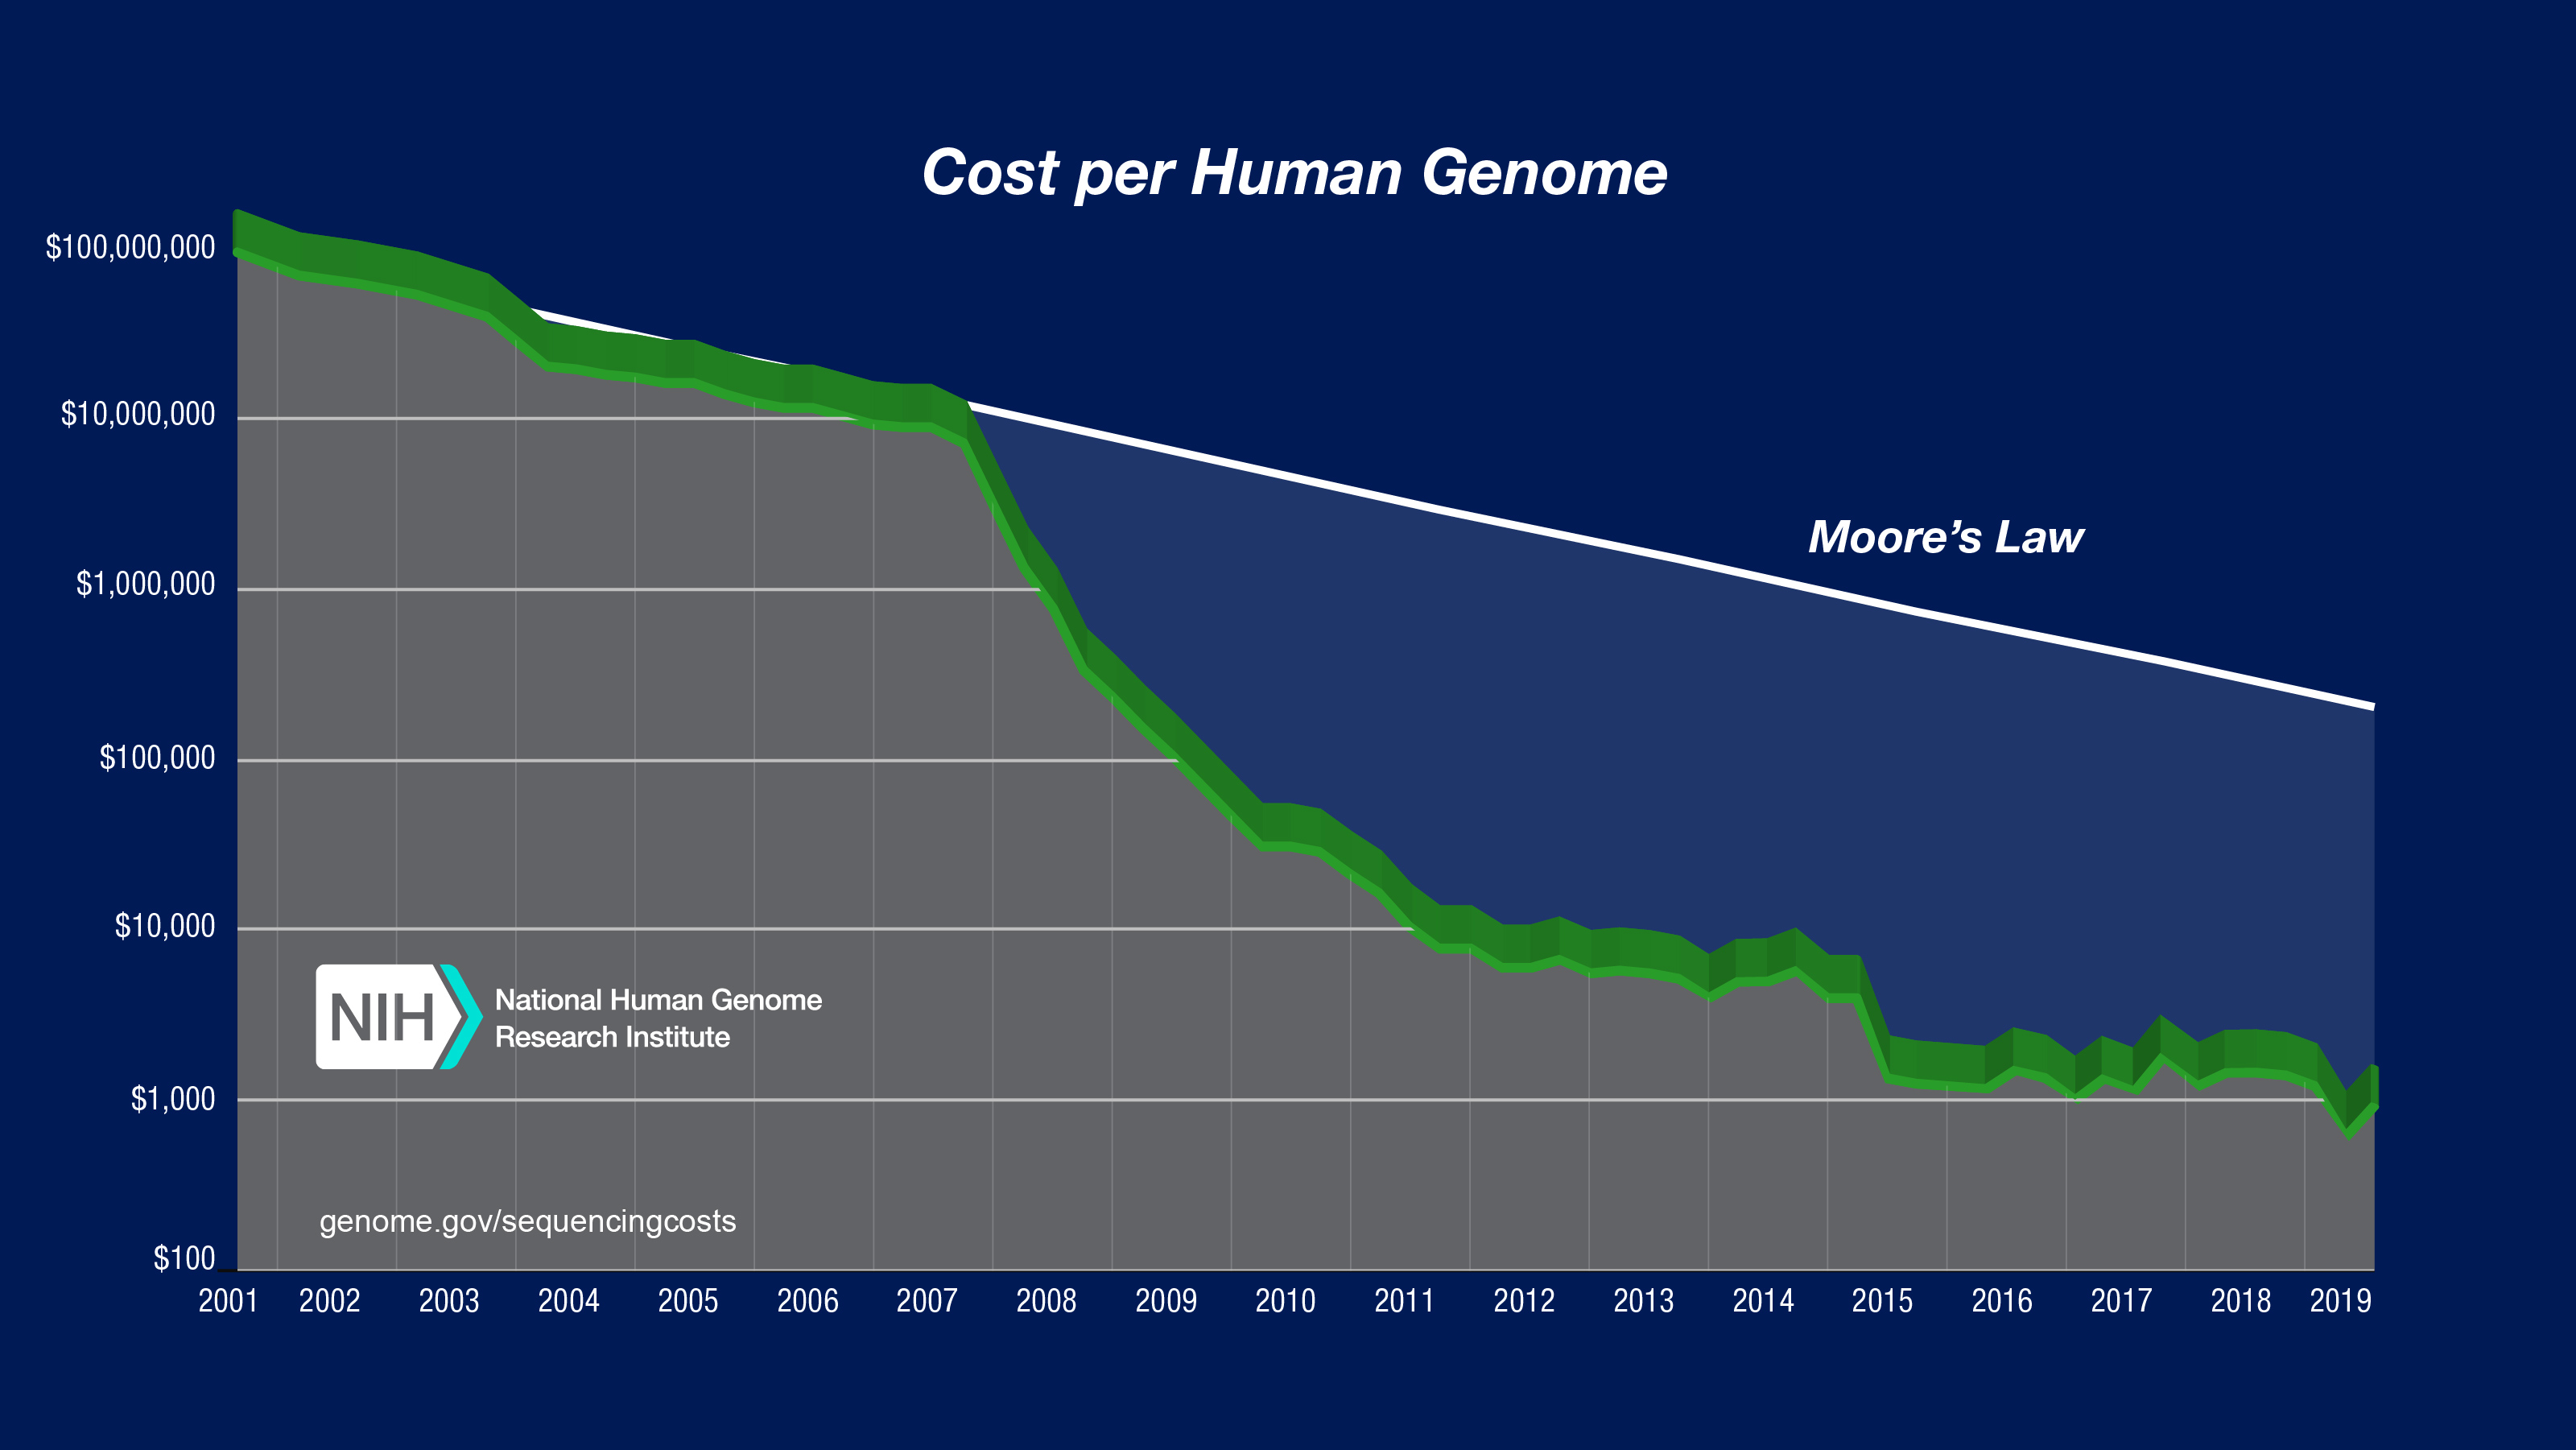
\includegraphics[width=.8\linewidth]{Sequencing_Cost_per_Genome_August2019.jpg}
    \caption{Sequencing costs since the Human Genome Project}
    \label{fig:seq}
\end{figure}
\subsection{Long vs Short reads}
In most cases long reads are more useful, as less assembly is required to reconstruct the full sequence, but there are drawbacks like higher sequencing error (single-molecule), or low throughput (Sanger). Longer reads can resolve \textbf{complex repeat sequences}, and large \textbf{structural variation} in the sequence (like translocations); the length of repeats are often ambiguous with short reads. Short reads however are prone to less error while being high-throughput, so they are still useful for most problems.

\section{Assembly}
Let's now take a look at two methods for sequence assembly: \textbf{overlap-layout-consensus} and \textbf{De Bruijn graphs}. These techniques both use graphs to model relationships between reads (see the note on Phylogeny for details on graphs), but differ in how they actually represent individual reads (as nodes vs edges).
\begin{figure}[h!]
    \centering
    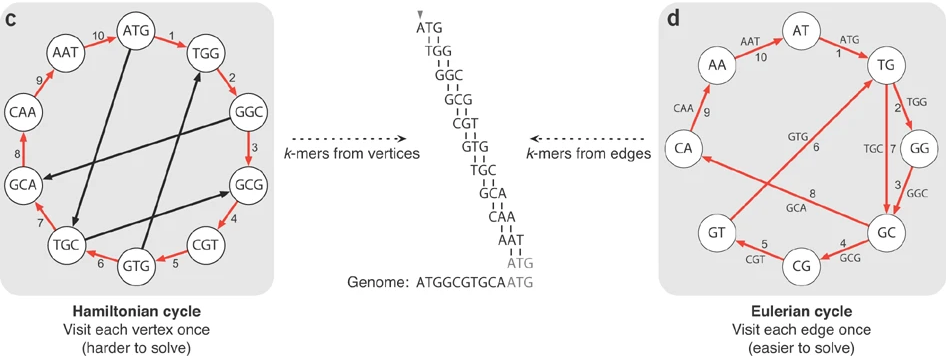
\includegraphics[width=\linewidth]{cycles.png}
    \caption{Hamiltonian vs Eulerian Cycles}
    \label{fig:cycle}
\end{figure}
\subsection{Overlap-Layout-Consensus}
In Overlap-Layout-Consensus (OLC), each read is represented as a node in the graph. Two nodes are connected by an edge if the reads share an overlap (e.g. the reads ATCG and CGTT overlap by two bp). A path in this graph represents a series of overlapping reads which form an assembled sequence. A path that connects all the nodes in the graph is known as a \textbf{Hamiltonian path}, which is a computationally difficult problem to solve.\\[10pt]
The OLC method works well with longer reads that vary in length (for example from single-molecule sequencing). This is because long reads are easier to join using sequence overlaps, and thus assembling longer contigs is simpler.
\subsection{De Bruijn Graphs}
In the De Bruijn graph method, node represent $(k-1)$-mers, where each read is size $k$. An edge connects two nodes if a read is composed of the overlap of those two $(k-1)$-mers. Thus the edges represent reads, and a path (like in overlap-layout-consensus) represents an assembled sequence. However, now the problem is finding a path that uses all edges, called an \textbf{Eulerian path}, which is computationally easier to solve.\\[10pt]
In these graphs, cycles represent repeats in the overall sequence, which can be hard to resolve (thus the advantage of longer reads!), as the number of repeats (the number of turns around the cycle) is ambiguous. Also, sequencing errors can cause issues with overlaps, which manifest as \textbf{bulges} in the graph.\\[10pt]
De Bruijn graphs are preferred for assembling short reads which are of similar size (length $k$), such as those from next generation sequencing. For short reads, it is easier to see how the reads cover the kmers of the assembly, rather than connect overlaps between sequences. Another reason is that the overall size of the graph size is not dependent on the number of reads (which is often large for short read sequencing). 

\subsection{Polishing}
Another method for assembly which is used with long-read sequencing is \textbf{polishing}. The initial step of this method uses OLC to create a rough draft of the assembly, which is then further improved. The polishing step involves aligning the long reads to the draft assembly for error correction (e.g. correcting bases in the assembly). The consenus assembly from OLC is used to resolve the overall structure of the assembly, while the polishing step resolves the details of the assembly. This step is necessary because of the noisy nature of long read sequencing, which can cause errors in the draft assembly which require polishing.

\subsection{Evaluating an assembly}
One method for evaluating a sequence assembly is the \textbf{N50} metric. The N50 value represents the minimum contig size threshold at which 50\% of assembled bases can be found. For example, if the N50 for an assembly is 1,000bp, then half the assembled bases can be found in contigs $\leq 1000$bp. N50 describes how fragmented an assembly is, and a \textit{larger N50 means a better assembly}. \textbf{CGAL} is another metric which represents the log-likelihood of each read in the assembly.

\section{Annotation}
Now let's look at the problem of annotating an assembled sequence. In particular we'll explore how to identify which open reading frames (ORFs) are genes.
\subsection{Find the ORFs}
We can start by identifying the ORFs in the assembled sequence. Each ORF starts with a \textbf{start codon} and ends with a \textbf{stop codon}, so we can scan the sequence and identify seqeunces between a start and stop codon. However, ORFs can overlap (and the start and stop codons must be in frame). Another issue is that \textit{not all ORFs are genes!} \\[10pt]
So how can we identify which ORFs are genes? One way is \textbf{homology search}, using BLAST or other tools to compare ORFs to characterized genes. But homology search can't identify novel genes, so we need a model that can classify an ORF as a gene \textit{de novo}!

\subsection{Probabilistic Models}
One way to approach this problem is with a probabilistic model, in this case a \textbf{Markov Model}. These models have a probability of generating any given sequence, and we can train them on sequences that we know are genes.\\[10pt]
Once the model is trained, when given an input sequence, the output is the probability of the model generating that sequence; thus high probability ORFs are likely genes. We can compare the model to a \textbf{null model}, which is trained on non-gene ORFs, and calculate the \textbf{log odds ratio} (see the note on Pairwise alignment).

\subsection{Markov Models}
One type of model used to classify ORFs is a \textbf{Fixed-Order Markov Model}. A \textit{k-th} order markov model uses the previous $k$ nucleotides as ``context":
\begin{figure}[h!]
    \centering
    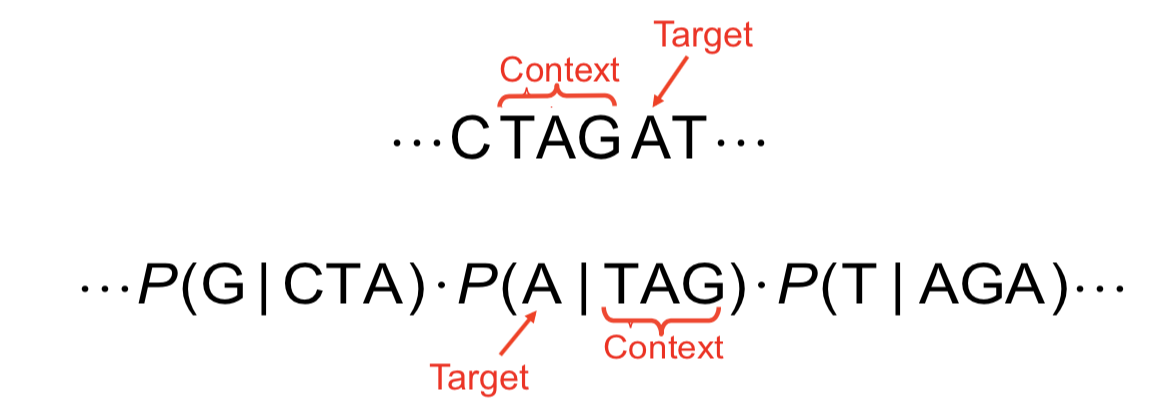
\includegraphics[width=.6\linewidth]{order_hmm.png}
    \caption{Context in a 3rd Order Markov Model}
    \label{fig:order}
\end{figure}

Fixed order models are relatively easy to train by counting the frequency of ($k+1$)-mers in the training sequences, and building a conditional probability table. However, some kmers may be undersampled, and often a nucleotide position may not depend on a fixed context.\\[10pt]
\textbf{Interpolated Markov Models} (used in the Glimmer 1.0) condition the probability of a nucleotide using a \textit{variable} number of previous positions. These models outperform fixed-order models, but they are slower to train and risk overfitting.\\[10pt]
Lastly, \textbf{Interpolated Context Models} (used in Glimmer 2.0) allow \textit{non-adjacent} bases in the context window to be used to predict the next base. The model determines which previous bases are most informative in predicting the next base by measuring the \textbf{mutual information} between each previous position and the current position in the sequence (see the note on Information Theory).

\begin{figure}[h]
    \centering
    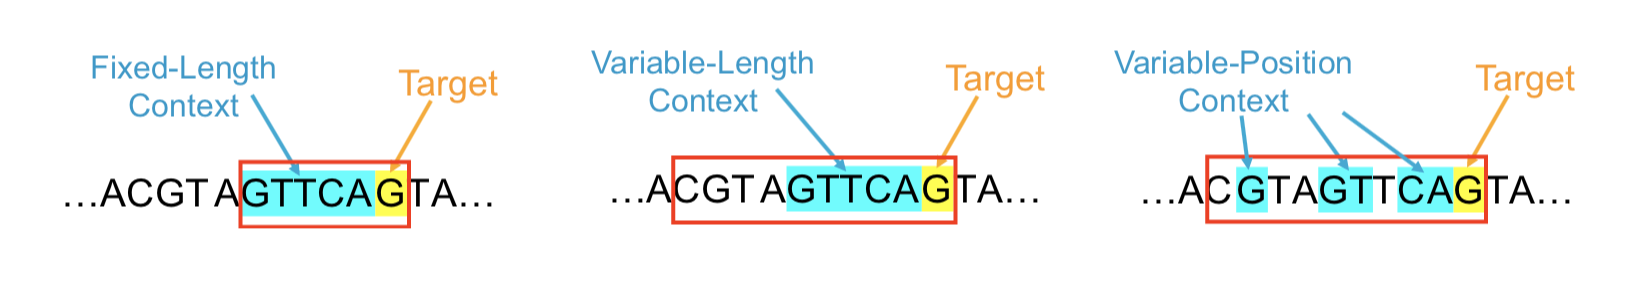
\includegraphics[width=\linewidth]{hmm_context.png}
    \caption{Types of sequence contexts}
    \label{fig:my_label}
\end{figure}

\subsection{HMM genefinders}
Another class of models for identifying and annotating genes (particularly in eukaryotes) are \textbf{hidden markov models (HMMs)} (see the note on probability for more details on HMMs). HMMs can be used to identify genes by modeling introns, exons, and other structural features of gene sequences using state and emission probabilities (hidden states $\rightarrow$ features like exons/introns, emissions $\rightarrow$ nucleotide sequence).\\[10pt]
The first groundbreaking HMM for gene annotation was GENSCAN (Burge and Karlin, 1997), which used multiple signal detectors in single HMM to find high probability genes from sequence. Another similar model, SNAP (Korf, 2004), was developed as a trainable and parameterizable HMM for gene detection.
\begin{figure}[h]
    \centering
    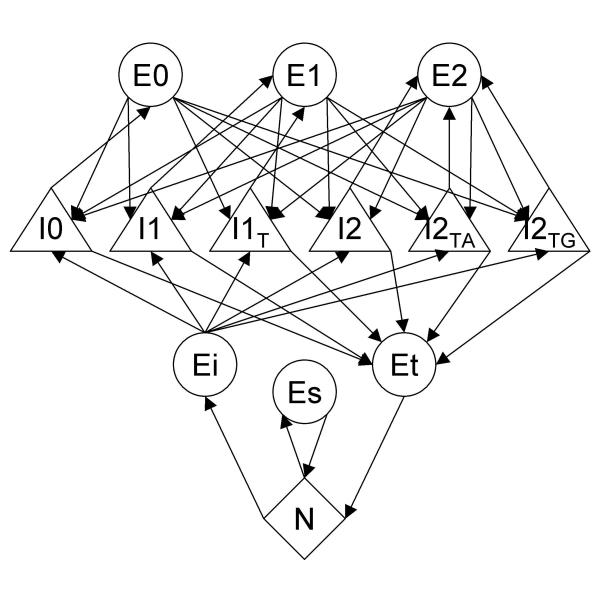
\includegraphics[width=.4\linewidth]{snap.jpg}
    \caption{SNAP model (Korf, 2004)}
    \label{fig:snap}
\end{figure}
\subsection{Homology Assignment}
Probabilistic models are useful for identifying novel genes, but often we have a sequence for a gene or protein which has been characterized before. In these cases, we can use \textbf{homology} to determine the protein product or gene identity. One method is to \textbf{BLAST} the sequence against a database and look for close matches. In the case of proteins, we can use methods like \textbf{PFAM}, which identify protein domains using sequence signatures. 

\section{Genome Browsers}
The purpose of genome browsers is to provide a simple method for presenting \textit{primary evidence from sequencing experiments} (using the logical format of a genomic coordinate scheme). We can use these browsers to examine how sequencing reads are distributed, which is a main source of evidence in an experiment. The browser also allows a user to visualize this data for \textbf{quality control} and downstream analysis.\\[10pt]
In the last section of this note, we'll discuss how genome browsers work, in particular how they efficiently explore large sequence data with various \textbf{indexing techniques}. Browsers like the \textbf{UCSC Browser}, \textbf{Integrative Genomics Viewer (IGV)}, and \textbf{JBrowse} interactively display sequences with annotations along with various sequence tools, which is useful for handling, analyzing, and presenting biological sequence data.
\subsection{Genome Indexing}
Let's look at a few methods for indexing genomes (or large sequences).

\subsubsection{Interval containers}
First we'll look at efficient methods for querying from \textbf{intervals}.
An interval in a genome sequence can be represented as a 2D point (start, end). Now, given two intervals, how can we tell if they overlap? two intervals $(a, b)$ and $(c, d)$ overlap if and only if the following conditions are true:
$$c \leq b\text{ AND }d\geq a$$
See figure \ref{fig:interval} to visualize why this is true.\\[10pt]
This condition can be visualized on a 2D coordinate system: first a point is reflected over the line $y=x$, and a rectangular region is drawn on the top left quadrant of the reflected point. All points in this region overlap with the interval of interest (see figure \ref{fig:interval}).\\[10pt]
Thus an overlap query is analogous to determining if a point is within this rectangular region. One data structure that can efficiently handle this query is a \textbf{Range tree}. Similar to a binary search tree (which is a 1D range tree), this data structure can run an overlap query in $O(\log(\log(N))$ time, and can be constructed in $(N\log N)$ time.
\begin{figure}[h]
    \centering
    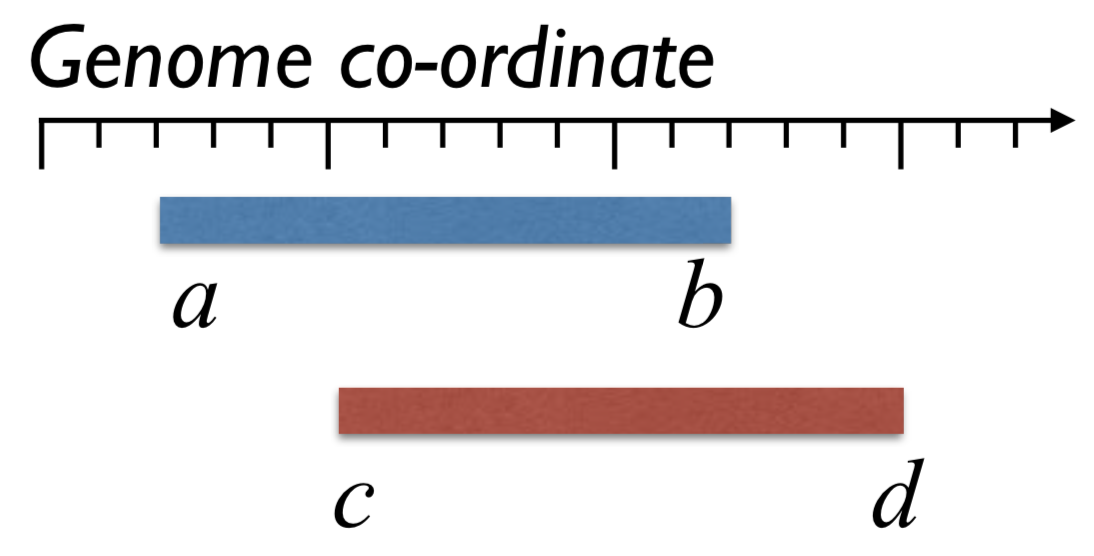
\includegraphics[width=.45\linewidth]{interval.png}
    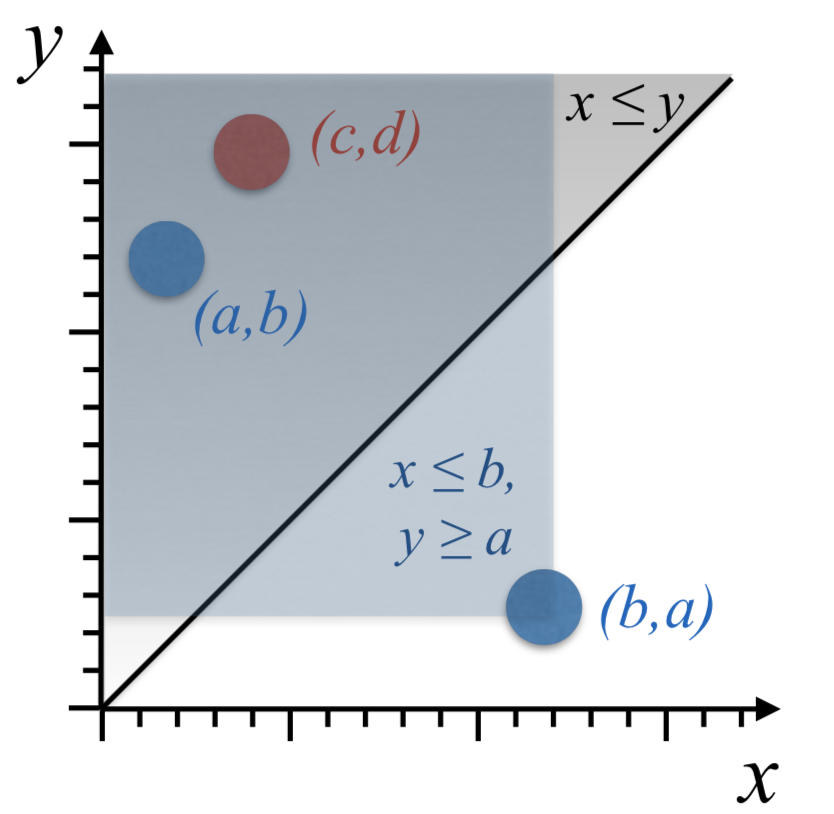
\includegraphics[width=.45\linewidth]{rtree.png}
    \caption{Example of overlapping intervals (left) and range of overlapping intervals (right)}
    \label{fig:interval}
\end{figure}\\
Another data structure that is more efficient that range trees in practice is a \textbf{Nested Containment List}. This data structure is similarly tree structured, where the each child is contained in the parent interval, while siblings have no containment relationship.\\[10pt]
Querying an NCList takes $O(\log N)$ time, while construction takes $O(N\log N)$ time. Though the asymptotic runtime is worse than range trees, in practice (in terms of magnitude of operations, etc.), nested containment lists tend to be much faster. \textit{Note}: nested containment lists are generally constructed with the idea that no intervals will be added or removed after the structure has initially been created (they are static, not dynamic, data structures).
\subsection{Sequence Indices}
Now let's look at methods to index a sequence and test for set membership, which, for example, can be useful for efficiently querying if a coordinate overlaps with annotations in a genomic region. We have already seen a couple of indexing methods (suffix trees and FM index [see notes on Pairwise Alignment and Information Theory]), so now we will focus on two \textbf{hash-based methods}. The important condition for both methods is that they have \textbf{\textit{good} hash functions}, which uniformly distribute hashed values and similar inputs have very different outputs. \\[10pt]
The first method, a \textbf{Bloom filter}, can be used to efficiently query if an item is part of a set. \textbf{False positives} are allowed, but never \textbf{false negatives} (that is, we can know for sure if an item is \textit{not} in a list, but we can't be sure that if it's in the set). First, we use a length $m$ array and $k$ hash functions. To add an item, we compute the $k$ hash values, which we treat as indices in the array, and set those positions to 1. Then to query for set membership, we can just check the $k$ positions again and see if they all have 1s!\\[10pt]
\begin{figure}[t]
    \centering
    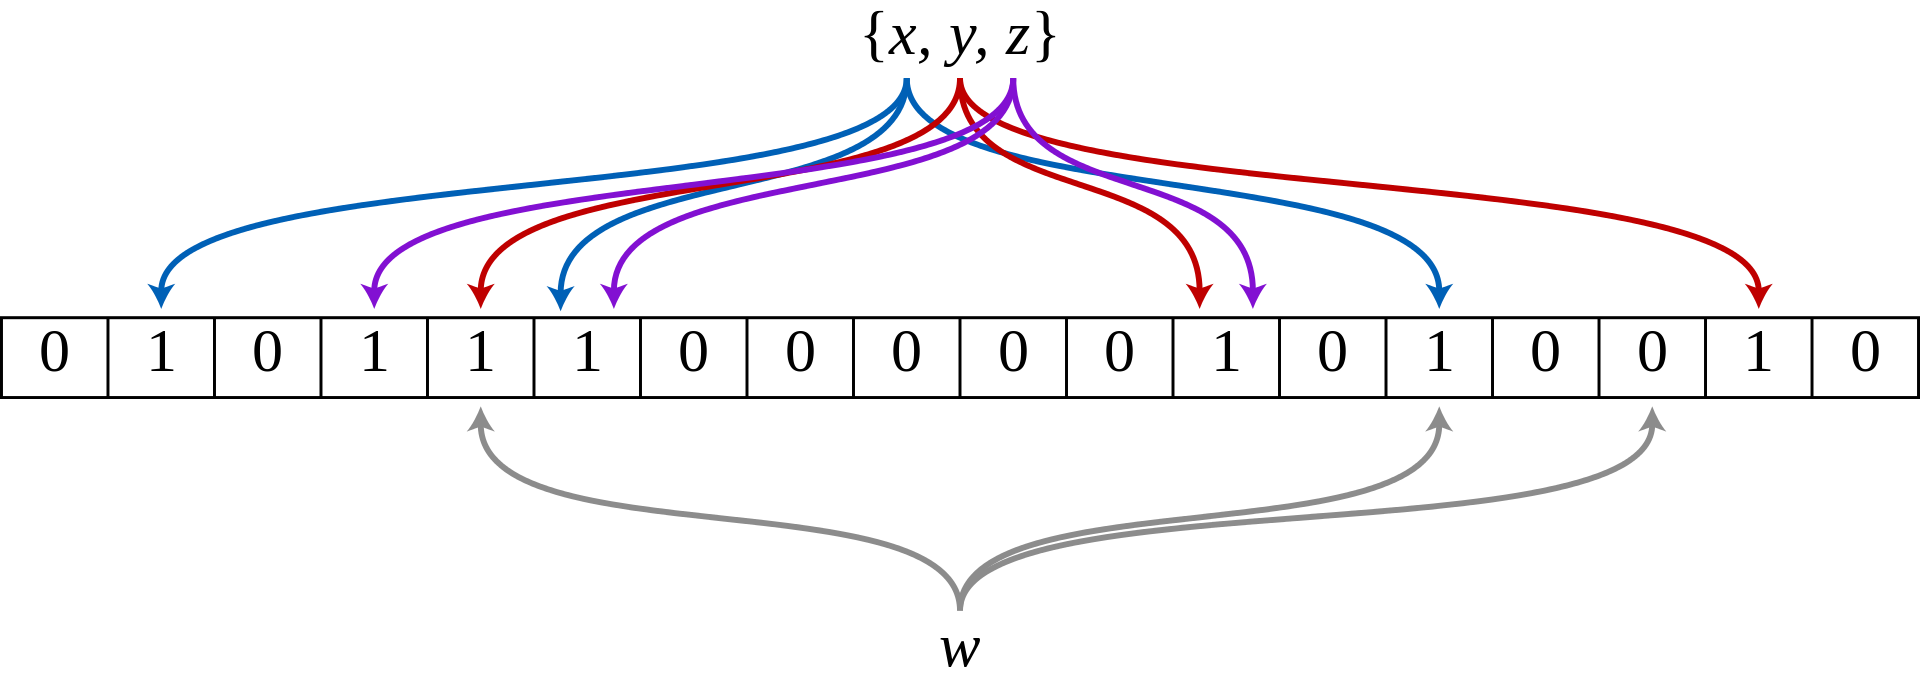
\includegraphics[width=.7\linewidth]{1920px-Bloom_filter.svg.png}
    \caption{A Bloom filter for set \{x,y,z\}, where $w$ is not in the set}
    \label{fig:my_label}
\end{figure}
\textbf{MinHash} is a technique to estimate the \textbf{Jaccard similarity coefficient}, which is the ratio of the intersection of two sets and the union of the sets:
$$J(A,B) = \frac{|A \cap B|}{|A \cup B|}$$
A Jaccard coefficient of 0 means the sets are disjoint, while a coefficient of 1 means the sets are identical. The MinHash method uses the following relationship between hash functions and the Jaccard coefficient:
$$P(h_{\min}(A) = h_{\min}(B)) = J(A,B)$$
where $h_{\min}(A)$ is the minimum hash value in set $A$. Thus to estimate the Jaccard coefficient, we can compute min hash value of both sets for many hash functions, and count how many yield equal minhash values.

\section{Summary}
Until this note, we assumed that we had sequences to analyze and align. But an important task in bioinformatics is assembling and annotating these sequences from raw sequence data. Algorithms and tools that have been developed for these tasks borrow techniques from graph theory and probability theory to efficiently build and annotate sequences. Lastly, once we have assembled sequences, we often want to visualize the annotations, assemblies, and alignments using genome browsers. These tools also use various techniques to efficiently compute information about the genome and present the data.
\end{document}


%topics not covered:
%names of assemblers
%glimmer3, overlapping orfs, ICM as a tree
%eukaryotic gene finders
%HMMs
%non protein coding rna homology (grammars)

%not sure how to write about the set intervals, hash based indices, etc